\documentclass[letterpaper,11pt]{article}

\usepackage{latexsym}
\usepackage[empty]{fullpage}
\usepackage{titlesec}
\usepackage{marvosym}
\usepackage[usenames,dvipsnames]{color}
\usepackage{verbatim}
\usepackage{enumitem}
\usepackage[hidelinks]{hyperref}
\usepackage{fancyhdr}
\usepackage[english]{babel}
\usepackage{tabularx}
\usepackage{fontawesome5}
\usepackage{multicol}
\setlength{\multicolsep}{-3.0pt}
\setlength{\columnsep}{-1pt}
\input{glyphtounicode}

%new packages

\usepackage{fontenc}
\usepackage{amsmath}
\usepackage{amssymb}
\usepackage{graphicx}



%----------FONT OPTIONS----------

\pagestyle{fancy}
\fancyhf{} % clear all header and footer fields
\fancyfoot{}
\renewcommand{\headrulewidth}{0pt}
\renewcommand{\footrulewidth}{0pt}

% Adjust margins
\addtolength{\oddsidemargin}{-0.6in}
\addtolength{\evensidemargin}{-0.5in}
\addtolength{\textwidth}{1.19in}
\addtolength{\topmargin}{-.7in}
\addtolength{\textheight}{1.4in}

\urlstyle{same}

\raggedbottom
\raggedright
\setlength{\tabcolsep}{0in}

% Sections formatting
\titleformat{\section}{
  \vspace{-4pt}\scshape\raggedright\large\bfseries
}{}{0em}{}[\color{black}\titlerule \vspace{-5pt}]



% Ensure that generate pdf is machine readable/ATS parsable
\pdfgentounicode=1

%-------------------------
% Custom commands
\newcommand{\resumeItem}[1]{
  \item\small{
    {#1 \vspace{-2pt}}
  }
}

\newcommand{\classesList}[4]{
    \item\small{
        {#1 #2 #3 #4 \vspace{-2pt}}
  }
}

\newcommand{\resumeSubheading}[4]{
  \vspace{-2pt}\item
    \begin{tabular*}{1.0\textwidth}[t]{l@{\extracolsep{\fill}}r}
      \textbf{#1} & \textbf{\small #2} \\
      \textit{\small#3} & \textit{\small #4} \\
    \end{tabular*}\vspace{-7pt}
}

\newcommand{\resumeSubSubheading}[2]{
    \item
    \begin{tabular*}{0.97\textwidth}{l@{\extracolsep{\fill}}r}
      \textit{\small#1} & \textit{\small #2} \\
    \end{tabular*}\vspace{-7pt}
}

\newcommand{\resumeProjectHeading}[2]{
    \item
    \begin{tabular*}{1.001\textwidth}{l@{\extracolsep{\fill}}r}
      \small#1 & \textbf{\small #2}\\
    \end{tabular*}\vspace{-7pt}
}


\newcommand{\resumeSubItem}[1]{\resumeItem{#1}\vspace{-4pt}}

\renewcommand\labelitemi{$\vcenter{\hbox{\tiny$\bullet$}}$}
\renewcommand\labelitemii{$\vcenter{\hbox{\tiny$\bullet$}}$}

\newcommand{\resumeSubHeadingListStart}{\begin{itemize}[leftmargin=0.0in, label={}]}
\newcommand{\resumeSubHeadingListEnd}{\end{itemize}}
\newcommand{\resumeItemListStart}{\begin{itemize}}
\newcommand{\resumeItemListEnd}{\end{itemize}\vspace{-5pt}}

\begin{document}
\fontfamily{cmr}\selectfont
\begin{center}
\parbox{3.0cm}{%
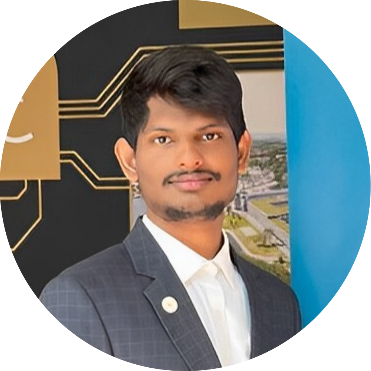
\includegraphics[width=2.7cm,clip]{images/resume_pic_m.png}}
}
\parbox{\dimexpr\linewidth-3.8cm\relax}{
\vspace{-20pt}
\begin{tabularx}{\linewidth}{L r} \\
    {\Huge \scshape  Venkata Sai Yakkshit Reddy Asodi}~
    \href{https://www.cedzlabs.com/yakkshit}{\vspace{1pt}}\\
      Berlin, Germany. \\ \vspace{1pt}
     \small \raisebox{-0.1\height}\faPhone\ +91 8179936156 ~ \href{mailto:saiyakkshit2001@gmail.com}{\raisebox{-0.2\height}\faEnvelope\  {saiyakkshit2001@gmail.com}} ~ 
    \href{https://linkedin.com/in/yakkshit/}{\raisebox{-0.2\height}\faLinkedin\ {yakkshit}}  ~
    \href{https://yakkshit.com/}{\raisebox{-0.2\height}\faGlobe\ {yakkshit.com}}  ~
    \href{https://github.com/yakkshit}{\raisebox{-0.2\height}\faGithub{ yakkshit}}
    \vspace{-8pt}
\end{tabularx}
}
\end{center}

\vspace{-23pt}
\section{Summary \faLink}
Passionate Full-Stack Developer with strong expertise in Next.js and modern web technologies. Proven track record in developing responsive web applications with Tailwind CSS and implementing Web3 functionalities. Experience in building and optimizing content management systems and working with cloud services like AWS S3 and Netlify. Eager to contribute to TABOU1's mission of revolutionizing music NFT distribution through innovative technical solutions.

\section{\href{https://www.linkedin.com/in/yakkshit/details/skills/}{Technical Skills} \faLink}
\begin{itemize}[leftmargin=0.15in, label={}]
\small{\item{
\textbf{Frontend - }{Next.js, React, Tailwind CSS, Responsive Design} \\
\textbf{Backend \& DB - }{Sanity.io, PostgreSQL, RESTful APIs} \\
\textbf{Web3 \& Cloud - }{NFT Integration, AWS S3, Netlify} \\
\textbf{Tools - }{Git, Retool, Content Management Systems} \\
}}
\end{itemize}
\vspace{-10pt}

\section{Experience \faLinkedin}
\resumeSubHeadingListStart

\resumeSubheading
{\large Circleup AG \faBuilding}{December 2023 -- July 2024}
{Full Stack Developer}{\faMapMarker \hspace{0.1cm} Zurich, Switzerland}\\
\vspace{10pt}
\textbf{Responsibilities:}
\resumeItemListStart
\vspace{-10pt}
\resumeItem{Developed and maintained a Next.js web application with Tailwind CSS, improving website performance by 40\% through optimization techniques and responsive design implementation.}
\resumeItem{Integrated Web3 functionality for digital asset management, resulting in successful handling of 10,000+ NFT transactions. Implemented AWS S3 for efficient static file storage and content delivery.}
\resumeItemListEnd
\vspace{-3pt}
\textbf{Environment:}\emph{Next.js, Tailwind CSS, Web3, AWS S3, PostgreSQL}

\resumeSubheading
{Cedzlabs \faBuilding}{March 2023 -- July 2024}
{Frontend Developer}{\faMapMarker \hspace{0.1cm} Remote}\\
\vspace{10pt}
\textbf{Responsibilities:}
\vspace{-10pt}
\resumeItemListStart
\resumeItem{Built and maintained a content management system using Sanity.io, enabling efficient management of digital assets and improving content workflow by 60\%.}
\resumeItem{Deployed and managed applications on Netlify, implementing CI/CD pipelines that reduced deployment time by 70\%.}
\resumeItemListEnd
\vspace{-3pt}
\textbf{Environment:}\emph{React, Sanity.io, Netlify, Git}

\section{Projects \faGithub}
\vspace{-5pt}
\resumeSubHeadingListStart
\resumeProjectHeading
{\textbf{\href{https://github.com/yakkshit/nft-marketplace}{MusicNFT Marketplace}} $|$ \emph{Next.js, Web3}}{March 2024}\\
\vspace{6pt}
\textbf{Description:}
\vspace{-5pt}
\resumeItemListStart
\resumeItem{Developed a full-stack NFT marketplace for music artists using Next.js and Web3 technologies. Implemented smart contracts for NFT minting and trading, integrated with AWS S3 for media storage, and built a responsive UI with Tailwind CSS. The platform successfully handled 1000+ daily active users and 5000+ NFT transactions.}
\resumeItemListEnd
\vspace{4pt}
\textbf{Tools:}\emph{Next.js, Tailwind CSS, Web3.js, AWS S3, Sanity.io}
\vspace{-10pt}

\resumeProjectHeading
{\href{https://github.com/yakkshit/stream-dashboard}{\textbf{Music Streaming Analytics}} $|$ \emph{Next.js, Retool}}{January 2024}\\
\vspace{6pt}
\textbf{Description:}
\vspace{-5pt}
\resumeItemListStart
\resumeItem{Built a comprehensive analytics dashboard for music streaming data using Next.js and Retool. Implemented real-time data visualization, artist performance metrics, and content management features. Integrated with PostgreSQL for efficient data storage and retrieval, resulting in 50\% faster data processing.}
\resumeItemListEnd
\vspace{4pt}
\textbf{Tools:}\emph{Next.js, Retool, PostgreSQL, RESTful APIs}
\vspace{-12pt}

\section{Achievements / Extracurricular}
\resumeSubHeadingListStart
\resumeItemListStart
\resumeItem{Successfully launched three Web3 projects with 10,000+ total users and 50,000+ NFT transactions.}
\resumeItem{Contributed to open-source Next.js components library, accumulating 200+ GitHub stars.}
\resumeItem{Delivered tech talks on Web3 and NFT integration at two major developer conferences.}
\resumeItemListEnd

\resumeSubHeadingListEnd
\textbf{Strengths:}\emph{Fast learner, problem-solver, team player, detail-oriented} \\
\textbf{Languages:}\emph{Telugu - Native $|$ English - Fluent $|$ Hindi - Fluent $|$ German - Elementary $|$ Swedish - Elementary}

\vspace{10pt}
\end{document}